\documentclass[11pt]{article}
% =====================================================================
% ALGEBRA 1 --- CHAPTER 4, SECTION 4-7: ARITHMETIC SEQUENCES
% Handout + worksheet (5 topics, 2 easy / 2 medium / 1 hard each)
% + fully detailed answer key.
% Copyright (c) 2026 FangMath.  All rights reserved.
% =====================================================================
\usepackage[letterpaper,margin=0.80in,top=0.70in,bottom=0.84in]{geometry}
\usepackage[T1]{fontenc}
\usepackage{amsmath,amssymb}
\usepackage{cancel}
\usepackage[table]{xcolor}
\usepackage[most]{tcolorbox}
\usepackage{enumitem}
\usepackage{pifont}
\usepackage{fancyhdr}
\usepackage{tikz}
\usetikzlibrary{calc,arrows.meta,decorations.pathreplacing}

\definecolor{ink}{RGB}{28,58,102}
\definecolor{inkpale}{RGB}{226,234,245}
\definecolor{sea}{RGB}{18,110,92}
\definecolor{seapale}{RGB}{224,241,236}
\definecolor{crim}{RGB}{170,45,45}
\definecolor{crimpale}{RGB}{251,230,228}
\definecolor{amber}{RGB}{184,120,16}
\definecolor{amberpale}{RGB}{253,243,222}
\definecolor{violet}{RGB}{95,60,140}
\definecolor{violetpale}{RGB}{237,231,246}
\definecolor{slate}{RGB}{92,102,118}

\pagestyle{fancy}
\fancyhf{}
\renewcommand{\headrulewidth}{0.4pt}
\renewcommand{\footrulewidth}{0.4pt}
\lhead{\small\itshape\color{ink} Algebra 1 \ $\cdot$ \ 4-7 Arithmetic Sequences}
\rhead{\small\itshape\color{ink}\leftmark}
\lfoot{\footnotesize\itshape \textcopyright\ 2026 FangMath}
\rfoot{\small\color{ink}\thepage}

\setlength{\parindent}{0pt}
\setlength{\parskip}{3pt}

\newcommand{\ans}[1]{\boxed{#1}}
\newcommand{\vans}[1]{\textbf{\textcolor{ink}{#1}}}
\newcommand{\rsn}[1]{\textcolor{slate}{\text{#1}}}
\newcommand{\mpos}[1]{\textcolor{sea}{#1}}
\newcommand{\mneg}[1]{\textcolor{crim}{#1}}
\newcommand{\A}[1]{A(#1)}

\newtcolorbox{keybox}[1][How To Do It]{colback=inkpale,colframe=ink,coltitle=white,
  colbacktitle=ink,fonttitle=\bfseries,title={#1},
  arc=2pt,boxrule=0.9pt,left=7pt,right=7pt,top=4pt,bottom=4pt,breakable}
\newtcolorbox{exbox}[1][\ding{43}\ \ Worked Example]{colback=seapale,colframe=sea,coltitle=white,
  colbacktitle=sea,fonttitle=\bfseries,title={#1},
  arc=2pt,boxrule=0.9pt,left=7pt,right=7pt,top=4pt,bottom=4pt,breakable}
\newtcolorbox{warnbox}[1][\ding{55}\ \ Common Mistake]{colback=crimpale,colframe=crim,
  coltitle=white,colbacktitle=crim,fonttitle=\bfseries,title={#1},
  arc=2pt,boxrule=0.9pt,left=7pt,right=7pt,top=4pt,bottom=4pt,breakable}
\newtcolorbox{notebox}[1][\ding{42}\ \ Note]{colback=amberpale,colframe=amber,
  coltitle=white,colbacktitle=amber,fonttitle=\bfseries,title={#1},
  arc=2pt,boxrule=0.9pt,left=7pt,right=7pt,top=4pt,bottom=4pt,breakable}
\newtcolorbox{deepbox}[1]{colback=violetpale,colframe=violet,coltitle=white,
  colbacktitle=violet,fonttitle=\bfseries,title={\ding{72}\ \ #1},
  arc=2pt,boxrule=0.9pt,left=7pt,right=7pt,top=4pt,bottom=4pt,breakable}

\newcounter{topicnum}
\newcommand{\topic}[2]{%
  \clearpage\refstepcounter{topicnum}\markboth{Topic \thetopicnum: #1}{Topic \thetopicnum: #1}%
  \vspace*{-4pt}\par\noindent
  \begin{tcolorbox}[colback=ink,colframe=ink,arc=3pt,
    left=12pt,right=12pt,top=7pt,bottom=7pt,boxrule=0pt]
  {\color{white}\bfseries\Large Topic \thetopicnum\ \ $\cdot$\ \ #1}\\[2pt]
  {\color{white}\itshape\small #2}
  \end{tcolorbox}\par\vspace{5pt}}

\newcommand{\banner}[3]{%
  \clearpage\markboth{#1}{#1}%
  \vspace*{-4pt}\par\noindent
  \begin{tcolorbox}[colback=#3,colframe=#3,arc=3pt,
    left=12pt,right=12pt,top=7pt,bottom=7pt,boxrule=0pt]
  {\color{white}\bfseries\Large #1}\\[2pt]
  {\color{white}\itshape\small #2}
  \end{tcolorbox}\par\vspace{5pt}}

\newcommand{\lvl}[3]{%
  \par\penalty-100\vspace{6pt}\noindent
  \begin{tcolorbox}[colback=#1!12,colframe=#1,arc=2pt,boxrule=0pt,
    leftrule=3.2pt,left=8pt,right=8pt,top=2.5pt,bottom=2.5pt]
  {\color{#1}\bfseries #2}\ \ {\color{slate}\small\itshape #3}
  \end{tcolorbox}\par\nopagebreak\vspace{2pt}}

\newcommand{\keyhead}[1]{%
  \par\vspace{9pt}\noindent
  \begin{tcolorbox}[colback=violet!12,colframe=violet,arc=2pt,boxrule=0pt,
    leftrule=3.2pt,left=8pt,right=8pt,top=3pt,bottom=3pt]
  {\color{violet}\bfseries #1}
  \end{tcolorbox}\par\vspace{2pt}}

% ---------- ruled work space ----------
\makeatletter
\newcommand{\worklines}[1]{\par\vspace{3pt}%
  \@tempcnta=0
  \@whilenum\@tempcnta<#1\do{%
    \noindent\textcolor{ink!25}{\rule{\linewidth}{0.5pt}}\par\vspace{16pt}%
    \advance\@tempcnta by 1}%
  \vspace{-10pt}}
\makeatother

% ---------- sequence with +d arrows:  \seqarrows{a}{b}{c}{d}{step} ----------
\newcommand{\seqarrows}[5]{%
\begin{tikzpicture}[x=1.35cm,y=1cm,baseline=0pt]
  \foreach \v/\i in {#1/0,#2/1,#3/2,#4/3}{
     \node[font=\large,ink] at (\i,0) {$\v$};
     \ifnum\i<3 \node[font=\large,ink] at ({\i+0.5},0) {,}; \fi }
  \node[font=\large,ink] at (3.55,0) {, \ \ldots};
  \foreach \i in {0,1,2}{
     \draw[crim,->,line width=1pt,shorten >=3pt,shorten <=3pt]
        ({\i+0.1},-0.22) to[bend right=45] ({\i+0.9},-0.22);
     \node[font=\small,crim] at ({\i+0.5},-0.72) {$#5$};}
\end{tikzpicture}}

\begin{document}

% =====================================================================
\thispagestyle{empty}
\begin{center}
\vspace*{0.2cm}
{\color{ink}\rule{\linewidth}{2.3pt}}\\[11pt]
{\color{ink}\bfseries\fontsize{29}{35}\selectfont Arithmetic Sequences}\\[6pt]
{\color{crim}\bfseries\fontsize{17}{21}\selectfont Algebra 1 \ $\cdot$ \ Chapter 4}\\[9pt]
{\color{ink}\rule{\linewidth}{2.3pt}}\\[11pt]
{\large Handout \ $\cdot$ \ 5 topics \ $\cdot$ \ 2 easy, 2 medium, 1 hard each\\[3pt]
25 practice problems \ $\cdot$ \ fully detailed answer key}
\end{center}

\vspace{0.35cm}
\begin{center}
\begin{tcolorbox}[colback=white,colframe=ink,width=0.94\linewidth,arc=3pt,boxrule=1.2pt,
  top=2pt,bottom=2pt]
\renewcommand{\arraystretch}{2.0}
\begin{tabular}{@{}p{1.7cm}p{6.4cm}p{1.5cm}p{3.4cm}@{}}
{\color{ink}\bfseries Name:} & \underline{\hspace{6.2cm}} &
{\color{ink}\bfseries Date:} & \underline{\hspace{3.2cm}}\\
\end{tabular}
\end{tcolorbox}
\end{center}

\vspace{0.3cm}
\begin{center}
\begin{tcolorbox}[colback=inkpale,colframe=ink,width=0.94\linewidth,arc=3pt,boxrule=1pt]
\renewcommand{\arraystretch}{1.42}
\begin{tabular}{@{}p{1.1cm}p{6.1cm}p{6.4cm}@{}}
\multicolumn{3}{@{}l@{}}{\color{ink}\bfseries\large Contents} \\[3pt]
\multicolumn{3}{@{}l@{}}{\color{crim}\bfseries The Handout \ \ {\normalsize\normalfont\itshape (read first)}}\\
\textbf{1} & Is it arithmetic? Find $d$ & {\footnotesize subtract consecutive terms} \\
\textbf{2} & The recursive formula & {\footnotesize where you start, and how you step} \\
\textbf{3} & The explicit formula & {\footnotesize $A(n)=A(1)+(n-1)d$} \\
\textbf{4} & Finding a term, finding $n$ & {\footnotesize forwards and backwards} \\
\textbf{5} & Word problems & {\footnotesize seats, savings, growth, profit} \\[5pt]
\multicolumn{3}{@{}l@{}}{\color{violet}\bfseries\large Detailed Answer Key \ \ {\normalsize\normalfont\itshape (at the end)}} \\
\end{tabular}
\end{tcolorbox}
\end{center}

\vspace{0.3cm}
\begin{center}
\begin{tcolorbox}[colback=amberpale,colframe=amber,width=0.94\linewidth,arc=3pt,boxrule=1pt]
\centering
{\small\textbf{Show all of your work in the space provided.} For every sequence problem, write
down \textbf{$A(1)$} and \textbf{$d$} first --- those two numbers determine everything else.}
\end{tcolorbox}
\end{center}

\vfill
\begin{center}
{\footnotesize\color{slate}\textcopyright\ 2026 \textbf{FangMath}. All rights reserved.}
\end{center}

% =====================================================================
% =====================================================================
\banner{The Handout}{Everything in 4-7, in the order it was taught}{crim}

\begin{keybox}[What makes a sequence \emph{arithmetic}]
A sequence is \textbf{arithmetic} when you get from each term to the next by
\textbf{adding the same number every time}. That number is the
\textbf{common difference}, written $d$.

\vspace{4pt}
\begin{center}
\seqarrows{70}{77}{84}{91}{+7}
\end{center}

\vspace{6pt}
\textbf{To test a sequence, subtract consecutive terms:}
\[
d=A(2)-A(1)=A(3)-A(2)=A(4)-A(3)=\cdots
\]
If all of those differences are equal, it \emph{is} arithmetic. If even one is different, it is
\textbf{not}.
\end{keybox}

\begin{exbox}[\ding{43}\ \ Once we determine it \emph{is} an arithmetic sequence \ldots]
\textbf{Sequence: \ $70,\ 77,\ 84,\ 91,\ \ldots$}

\vspace{3pt}
\textbf{Step 1 --- find the first term.}
\[
A(1)=70
\]
\textbf{Step 2 --- write how the second term comes from the first.}
\[
A(2)=A(1)+7
\]
\textbf{Step 3 --- generalise. This is the \emph{recursive formula}.}
\begin{center}
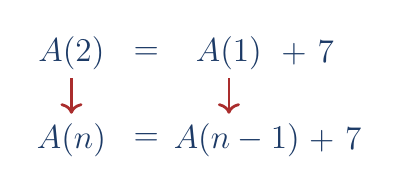
\begin{tikzpicture}[x=1cm,y=0.9cm]
  \node[font=\large,ink] at (0,0.6) {$A(2)$};
  \node[font=\large,ink] at (0.95,0.6) {$=$};
  \node[font=\large,ink] at (2.0,0.6) {$A(1)$};
  \node[font=\large,ink] at (3.0,0.6) {$+\ 7$};
  \draw[crim,->,line width=1pt] (0,0.25)--(0,-0.25);
  \draw[crim,->,line width=1pt] (2.0,0.25)--(2.0,-0.25);
  \node[font=\large,ink] at (0,-0.62) {$A(n)$};
  \node[font=\large,ink] at (0.95,-0.62) {$=$};
  \node[font=\large,ink] at (2.1,-0.62) {$A(n-1)$};
  \node[font=\large,ink] at (3.35,-0.62) {$+\ 7$};
\end{tikzpicture}
\end{center}
\[
\ans{A(1)=70, \qquad A(n)=A(n-1)+7, \quad n\ge 2}
\]

\vspace{3pt}
\vans{Why $n\ge2$?} \ The formula tells you how to get a term from the \emph{one before it}.
There is no term before $A(1)$, so the rule only makes sense from the second term onward.
\end{exbox}

\begin{exbox}[\ding{43}\ \ Your turn --- same three steps]
\textbf{Sequence (a): \ $3,\ 9,\ 15,\ 21,\ \ldots$}

\vspace{3pt}
\begin{center}
\seqarrows{3}{9}{15}{21}{+6}
\end{center}

\vspace{5pt}
\begin{tabular}{@{}p{5.0cm} p{9.5cm}@{}}
\textbf{Step 1.} First term & $A(1)=3$\\[3pt]
\textbf{Step 2.} Second term & $A(2)=A(1)+6$\\[3pt]
\textbf{Step 3.} Recursive formula & $A(n)=A(n-1)+6, \quad n\ge2$\\
\end{tabular}
\end{exbox}

% ---------------------------------------------------------------
\begin{deepbox}{Where the explicit formula comes from}
The recursive formula is fine for finding the \emph{next} term --- but to find $A(100)$ you would
have to compute all $99$ terms before it. Here is how to get a formula that jumps straight there.

\vspace{5pt}
\textbf{Write out the chain of recursive statements and add them all up.}
\begin{align*}
A(1) &= A(1)\\
A(2) &= A(1)+7\\
A(3) &= A(2)+7\\
A(4) &= A(3)+7\\
A(5) &= A(4)+7\\[-4pt]
\hline
\end{align*}
\vspace{-14pt}
\[
A(1)+A(2)+A(3)+A(4)+A(5)
\;=\;
A(1)+\Big[A(1)+A(2)+A(3)+A(4)\Big]+\underbrace{7+7+7+7}_{4\ \text{sevens}}
\]

\vspace{4pt}
\textbf{Now subtract $A(1)$, $A(2)$, $A(3)$ and $A(4)$ from both sides.}
Almost everything cancels:
\[
\cancel{A(1)}+\cancel{A(2)}+\cancel{A(3)}+\cancel{A(4)}+A(5)
=A(1)+\cancel{A(1)}+\cancel{A(2)}+\cancel{A(3)}+\cancel{A(4)}+4\cdot 7
\]
\[
\ans{A(5)=A(1)+4\cdot 7}
\]

\vspace{5pt}
\textbf{Read the pattern.} To reach the \textbf{5th} term you added $7$ exactly \textbf{4} times.
To reach the $n$th term you add $d$ exactly $n-1$ times:
\begin{center}
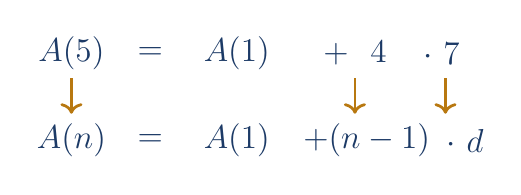
\begin{tikzpicture}[x=1cm,y=0.9cm]
  \node[font=\large,ink] at (0,0.55) {$A(5)$};
  \node[font=\large,ink] at (1.0,0.55) {$=$};
  \node[font=\large,ink] at (2.1,0.55) {$A(1)$};
  \node[font=\large,ink] at (3.6,0.55) {$+\ \ 4$};
  \node[font=\large,ink] at (4.7,0.55) {$\cdot\ 7$};
  \draw[amber,->,line width=1pt] (0,0.2)--(0,-0.3);
  \draw[amber,->,line width=1pt] (3.6,0.2)--(3.6,-0.3);
  \draw[amber,->,line width=1pt] (4.75,0.2)--(4.75,-0.3);
  \node[font=\large,ink] at (0,-0.68) {$A(n)$};
  \node[font=\large,ink] at (1.0,-0.68) {$=$};
  \node[font=\large,ink] at (2.1,-0.68) {$A(1)$};
  \node[font=\large,ink] at (3.75,-0.68) {$+(n-1)$};
  \node[font=\large,ink] at (5.0,-0.68) {$\cdot\ d$};
\end{tikzpicture}
\end{center}

\begin{center}
\begin{tcolorbox}[colback=white,colframe=violet,arc=2pt,boxrule=1.4pt,width=0.8\linewidth]
\centering
{\large \textbf{Explicit formula:} \qquad $A(n)=A(1)+(n-1)\,d$}
\end{tcolorbox}
\end{center}
For our sequence, $A(1)=70$ and $d=7$, so $A(n)=70+(n-1)\cdot 7$.
\end{deepbox}

\begin{notebox}[\ding{42}\ \ A shorter way to see the same thing]
Instead of adding all the equations, just substitute down the chain:
\begin{align*}
A(5)&=A(4)+7\\
&=\big[A(3)+7\big]+7 = A(3)+2\cdot7\\
&=\big[A(2)+7\big]+2\cdot 7 = A(2)+3\cdot 7\\
&=\big[A(1)+7\big]+3\cdot 7 = A(1)+4\cdot 7
\end{align*}
\vans{Count the steps, not the terms.} Going from term $1$ to term $5$ takes \textbf{4} steps ---
which is exactly why the formula says $n-1$ and not $n$.
\end{notebox}

\begin{center}
\begin{tcolorbox}[colback=inkpale,colframe=ink,width=0.97\linewidth,arc=3pt,boxrule=1.1pt]
{\color{ink}\bfseries\large The two formulas side by side}\par\vspace{4pt}
\renewcommand{\arraystretch}{1.5}
\begin{center}
\begin{tabular}{@{}p{3.3cm} p{5.2cm} p{5.8cm}@{}}
& \textbf{Recursive} & \textbf{Explicit} \\ \hline
\textbf{Formula} & $A(1)=\underline{\hspace{0.9cm}}$ \newline
 $A(n)=A(n-1)+d,\ n\ge2$ & $A(n)=A(1)+(n-1)d$ \\
\textbf{Says} & ``add $d$ to the term before'' & ``start at $A(1)$, add $d$ \ $(n-1)$ times'' \\
\textbf{Best for} & the \emph{next} term & a \emph{faraway} term, like $A(100)$ \\
\textbf{Must include} & \textbf{both} $A(1)$ and the rule & nothing else --- it stands alone \\
\end{tabular}
\end{center}
\end{tcolorbox}
\end{center}

\begin{warnbox}[\ding{55}\ \ The three mistakes that cost the most points]
\begin{enumerate}[leftmargin=1.7em,nosep,itemsep=3pt]
\item \textbf{Writing $(n)$ instead of $(n-1)$} in the explicit formula. Getting to term $n$ takes
$n-1$ steps. Test it: does your formula give the right \emph{first} term when $n=1$?
\item \textbf{Giving a recursive formula without $A(1)$.} ``$A(n)=A(n-1)+6$'' describes infinitely
many different sequences. \vans{The starting value is part of the answer.}
\item \textbf{Getting the sign of $d$ wrong on a decreasing sequence.} For $20,17,14,\ldots$ the
common difference is $\mneg{-3}$, not $3$. Always compute $d$ as \textbf{later term minus earlier
term}.
\end{enumerate}
\end{warnbox}

% =====================================================================
\topic{Is It Arithmetic? Find the Common Difference}{Subtract consecutive terms and compare}

\begin{keybox}
Compute $A(2)-A(1)$, then $A(3)-A(2)$, then $A(4)-A(3)$.
\begin{itemize}[leftmargin=1.5em,nosep,itemsep=2pt]
\item All the same $\Rightarrow$ \mpos{arithmetic}, and that common value is $d$.
\item Not all the same $\Rightarrow$ \mneg{not arithmetic}.
\end{itemize}
\textbf{Always subtract in the same direction:} later term $-$ earlier term.
\end{keybox}

\begin{exbox}
\textbf{Is $\ 70,\ 77,\ 84,\ 91,\ \ldots$ arithmetic? If so, find $d$.}
\[
77-70=7, \qquad 84-77=7, \qquad 91-84=7
\]
All three differences are equal, so
\[
\ans{\text{Yes --- arithmetic, with } d=7}
\]
\end{exbox}

\lvl{sea}{1. \ EASY}{}
Is $\ 5,\ 12,\ 19,\ 26,\ \ldots$ arithmetic? If so, state $d$.
\worklines{3}

\lvl{sea}{2. \ EASY}{a decreasing sequence}
Is $\ 20,\ 17,\ 14,\ 11,\ \ldots$ arithmetic? If so, state $d$.
\worklines{3}

\lvl{amber}{3. \ MEDIUM}{fractions}
Is $\ \dfrac12,\ 1,\ \dfrac32,\ 2,\ \ldots$ arithmetic? If so, state $d$.
\worklines{3}

\lvl{amber}{4. \ MEDIUM}{careful --- this one is a trap}
Is $\ 2,\ 4,\ 8,\ 16,\ \ldots$ arithmetic? Explain how you know.
\worklines{4}

\lvl{crim}{5. \ HARD}{solve for the unknown}
For what value of $k$ is $\ 3k-1,\ \ 2k+3,\ \ 5k-4\ $ an arithmetic sequence? Then state $d$.
\worklines{7}

% =====================================================================
\topic{The Recursive Formula}{Where you start, and how you step}

\begin{keybox}
A recursive formula has \textbf{two parts}, and you need both:
\begin{center}
\begin{tcolorbox}[colback=white,colframe=ink,arc=2pt,boxrule=1.2pt,width=0.78\linewidth]
\centering
$A(1)=\text{first term}$ \qquad and \qquad $A(n)=A(n-1)+d, \quad n\ge2$
\end{tcolorbox}
\end{center}
For a \textbf{decreasing} sequence $d$ is negative --- write $A(n)=A(n-1)+(-8)$ or
$A(n)=A(n-1)-8$.
\end{keybox}

\begin{exbox}
\textbf{Write the recursive formula for $\ 3,\ 9,\ 15,\ 21,\ \ldots$}

\vspace{3pt}
\begin{tabular}{@{}p{4.6cm} p{9.6cm}@{}}
\textbf{Step 1.} First term & $A(1)=3$\\[3pt]
\textbf{Step 2.} Second term & $A(2)=A(1)+6$\\[3pt]
\textbf{Step 3.} Generalise & $A(n)=A(n-1)+6$\\
\end{tabular}
\[
\ans{A(1)=3, \qquad A(n)=A(n-1)+6, \quad n\ge 2}
\]
\end{exbox}

\lvl{sea}{6. \ EASY}{}
Write the recursive formula for $\ 4,\ 11,\ 18,\ 25,\ \ldots$
\worklines{3}

\lvl{sea}{7. \ EASY}{decreasing}
Write the recursive formula for $\ 100,\ 92,\ 84,\ 76,\ \ldots$
\worklines{3}

\lvl{amber}{8. \ MEDIUM}{run the formula forwards}
A sequence is given by $\ A(1)=-4\ $ and $\ A(n)=A(n-1)+9$ for $n\ge2$. List the first five terms.
\worklines{4}

\lvl{amber}{9. \ MEDIUM}{decimals}
Write the recursive formula for $\ 2.5,\ 4,\ 5.5,\ 7,\ \ldots$
\worklines{3}

\lvl{crim}{10. \ HARD}{}
A sequence has $A(1)=12$ and $A(n)=A(n-1)-5$ for $n\ge2$.
\begin{enumerate}[label=\textbf{(\alph*)},leftmargin=2.1em,nosep,itemsep=2pt]
\item List terms until you reach the first negative one.
\item Which term is it? State both $n$ and the value.
\end{enumerate}
\worklines{6}

% =====================================================================
\topic{The Explicit Formula}{$A(n)=A(1)+(n-1)d$}

\begin{keybox}
\begin{center}
\begin{tcolorbox}[colback=white,colframe=ink,arc=2pt,boxrule=1.3pt,width=0.62\linewidth]
\centering
{\large $A(n)=A(1)+(n-1)\,d$}
\end{tcolorbox}
\end{center}
\begin{enumerate}[leftmargin=1.7em,nosep,itemsep=2pt]
\item Find $A(1)$ and $d$.
\item Substitute them --- \textbf{do not substitute $n$}.
\item Simplify by distributing, if the question asks for simplest form.
\item \textbf{Check with $n=1$:} your formula must give back the first term.
\end{enumerate}
\end{keybox}

\begin{exbox}
\textbf{Write the explicit formula for $\ 70,\ 77,\ 84,\ 91,\ \ldots$, then simplify.}

\vspace{2pt}
Here $A(1)=70$ and $d=7$:
\begin{align*}
A(n) &= A(1)+(n-1)d\\
&= 70+(n-1)\cdot 7 && \rsn{substitute}\\
&= 70+7n-7 && \rsn{distribute}\\
&= 7n+63
\end{align*}
\[
\ans{A(n)=70+7(n-1)=7n+63}
\]
\emph{Check $n=1$:} $\ 7(1)+63=70$ \ding{51} \quad \emph{Check $n=3$:} $\ 21+63=84$ \ding{51}
\end{exbox}

\lvl{sea}{11. \ EASY}{}
Write and simplify the explicit formula for $\ 3,\ 9,\ 15,\ 21,\ \ldots$
\worklines{4}

\lvl{sea}{12. \ EASY}{decreasing}
Write and simplify the explicit formula for $\ 20,\ 17,\ 14,\ 11,\ \ldots$
\worklines{4}

\lvl{amber}{13. \ MEDIUM}{given $A(1)$ and $d$}
Write and simplify the explicit formula for the sequence with $A(1)=-7$ and $d=4$.
\worklines{4}

\lvl{amber}{14. \ MEDIUM}{recursive $\to$ explicit}
A sequence is given recursively by $A(1)=8$ and $A(n)=A(n-1)+5$. Write its \textbf{explicit}
formula in simplest form.
\worklines{4}

\lvl{crim}{15. \ HARD}{fractions, both formulas}
For $\ \dfrac14,\ \dfrac34,\ \dfrac54,\ \dfrac74,\ \ldots$ write \textbf{(a)} the recursive
formula and \textbf{(b)} the explicit formula, simplified into a single fraction.
\worklines{5}

% =====================================================================
\topic{Finding a Term, Finding $n$}{Forwards and backwards}

\begin{keybox}
\textbf{Forwards --- ``find $A(20)$''.} \ Substitute $n=20$ into the explicit formula.

\vspace{3pt}
\textbf{Backwards --- ``which term equals $99$?''} \ Set the explicit formula \emph{equal} to $99$
and solve the equation for $n$.
\begin{center}
\begin{tcolorbox}[colback=crimpale,colframe=crim,arc=2pt,boxrule=1pt,width=0.94\linewidth]
\centering
\textbf{$n$ must come out a positive whole number.} If it does not, the value is not in the
sequence.
\end{tcolorbox}
\end{center}
\end{keybox}

\begin{exbox}
\textbf{For $\ 70,\ 77,\ 84,\ \ldots$, find $A(20)$.}
\begin{align*}
A(20) &= A(1)+(20-1)d\\
&= 70+19\cdot 7 && \rsn{\textbf{19} steps, not 20}\\
&= 70+133 = 203
\end{align*}
\[
\ans{A(20)=203}
\]
\end{exbox}

\lvl{sea}{16. \ EASY}{}
A sequence has $A(1)=5$ and $d=3$. Find $A(10)$.
\worklines{3}

\lvl{sea}{17. \ EASY}{}
For $\ 4,\ 11,\ 18,\ 25,\ \ldots$ find $A(12)$.
\worklines{3}

\lvl{amber}{18. \ MEDIUM}{negative $d$}
For $\ 8,\ 5,\ 2,\ -1,\ \ldots$ find $A(25)$.
\worklines{4}

\lvl{amber}{19. \ MEDIUM}{work backwards}
For $\ 3,\ 9,\ 15,\ 21,\ \ldots$, which term is equal to $99$?
\worklines{5}

\lvl{crim}{20. \ HARD}{two terms given}
In an arithmetic sequence, $A(4)=19$ and $A(9)=44$.
\begin{enumerate}[label=\textbf{(\alph*)},leftmargin=2.1em,nosep,itemsep=2pt]
\item Find $d$. \qquad \textbf{(b)} Find $A(1)$. \qquad \textbf{(c)} Write the explicit formula.
\end{enumerate}
\worklines{8}

% =====================================================================
\topic{Word Problems}{Read the story, find $A(1)$ and $d$}

\begin{keybox}
Every arithmetic word problem gives you the same two things in disguise:
\begin{center}
\renewcommand{\arraystretch}{1.4}
\begin{tabular}{@{}p{5.2cm} p{9.2cm}@{}}
\textbf{The starting amount} & becomes $A(1)$ \\
\textbf{``each'' / ``every'' / ``per''} & becomes $d$ \\
\end{tabular}
\end{center}
Then decide which question is being asked: \textbf{find a term} (substitute $n$) or
\textbf{find $n$} (solve an equation). \vans{Answer in a sentence, with units.}
\end{keybox}

\begin{exbox}
\textbf{A theater has $22$ seats in the first row, and each row after has $3$ more seats than the
row before. How many seats are in row $15$?}

\vspace{2pt}
$A(1)=22$ (first row) and $d=3$ (each row after).
\begin{align*}
A(15) &= 22+(15-1)\cdot 3 = 22+14\cdot3 = 22+42 = 64
\end{align*}
\[
\ans{\text{Row } 15 \text{ has } 64 \text{ seats.}}
\]
\end{exbox}

\lvl{sea}{21. \ EASY}{}
Jaden deposits \$25 in week $1$. Each week after, he deposits \$15 more than the week before.
How much does he deposit in week $6$?
\worklines{3}

\lvl{sea}{22. \ EASY}{}
A sapling is $40$ cm tall when planted and grows $6$ cm each year. Write an explicit formula for
its height after $n$ years, then find its height after $12$ years.
\worklines{3}

\lvl{amber}{23. \ MEDIUM}{}
A gym charges a \$75 joining fee plus \$30 each month. Write a formula for the total paid after
$n$ months, then find the total after $18$ months.
\worklines{4}

\lvl{amber}{24. \ MEDIUM}{work backwards}
Logs are stacked with $30$ in the bottom row, and each row above has $2$ fewer logs.
Which row has exactly $4$ logs?
\worklines{4}

\lvl{crim}{25. \ HARD}{}
A company's profit was \$12{,}000 in year $1$ and grew by the same amount each year. In year $7$
the profit was \$30{,}000.
\begin{enumerate}[label=\textbf{(\alph*)},leftmargin=2.1em,nosep,itemsep=2pt]
\item Find $d$. \qquad \textbf{(b)} Write the explicit formula.
\item In which year does the profit \textbf{first exceed} \$50{,}000?
\end{enumerate}
\worklines{7}

% =====================================================================
% =====================================================================
\banner{Detailed Answer Key}{Every step shown, every answer checked}{violet}

\begin{center}
\begin{tcolorbox}[colback=violetpale,colframe=violet,width=0.98\linewidth,arc=3pt,boxrule=1pt]
{\color{violet}\bfseries\large Answers at a glance}\par\vspace{5pt}
\renewcommand{\arraystretch}{1.38}\setlength{\tabcolsep}{4pt}
{\small
\begin{tabular}{@{}p{0.8cm}p{6.0cm}p{0.8cm}p{6.4cm}@{}}
\textbf{1.} & Yes, $d=7$ & \textbf{14.} & $A(n)=8+5(n-1)=5n+3$\\
\textbf{2.} & Yes, $d=-3$ & \textbf{15.} & $A(n)=A(n-1)+\tfrac12$; \ $\tfrac{2n-1}{4}$\\
\textbf{3.} & Yes, $d=\tfrac12$ & \textbf{16.} & $A(10)=32$\\
\textbf{4.} & No --- differences $2,4,8$ & \textbf{17.} & $A(12)=81$\\
\textbf{5.} & $k=\tfrac{11}{4}$, \ $d=\tfrac54$ & \textbf{18.} & $A(25)=-64$\\
\textbf{6.} & $A(1)=4$; $A(n)=A(n-1)+7$ & \textbf{19.} & the $17$th term\\
\textbf{7.} & $A(1)=100$; $A(n)=A(n-1)-8$ & \textbf{20.} & $d=5$, $A(1)=4$, $A(n)=5n-1$\\
\textbf{8.} & $-4,\,5,\,14,\,23,\,32$ & \textbf{21.} & \$100\\
\textbf{9.} & $A(1)=2.5$; $A(n)=A(n-1)+1.5$ & \textbf{22.} & $H=40+6n$; \ $112$ cm\\
\textbf{10.} & $A(4)=-3$, the 4th term & \textbf{23.} & $T=75+30n$; \ \$615\\
\textbf{11.} & $A(n)=3+6(n-1)=6n-3$ & \textbf{24.} & row $14$\\
\textbf{12.} & $A(n)=20-3(n-1)=23-3n$ & \textbf{25.} & $d=3000$; $3000n+9000$; year $14$\\
\textbf{13.} & $A(n)=-7+4(n-1)=4n-11$ & &\\
\end{tabular}}
\end{tcolorbox}
\end{center}

% ---------------------------------------------------------------
\keyhead{Topic 1 \ \ $\cdot$ \ \ Is It Arithmetic? Find $d$}

\textbf{1.} \ $12-5=7$, \ $19-12=7$, \ $26-19=7$. All equal, so
$\ans{\text{yes, arithmetic with } d=7}$.

\vspace{3pt}
\textbf{2.} \ $17-20=-3$, \ $14-17=-3$, \ $11-14=-3$.
\[
\ans{\text{Yes, arithmetic with } d=-3}
\]
\vans{The sign matters.} The terms are going \emph{down}, so $d$ is negative.

\vspace{3pt}
\textbf{3.} \ $1-\tfrac12=\tfrac12$, \ $\tfrac32-1=\tfrac12$, \ $2-\tfrac32=\tfrac12$.
\[
\ans{\text{Yes, arithmetic with } d=\tfrac12}
\]

\vspace{4pt}
\textbf{4.} \ Compute the differences:
\[
4-2=2, \qquad 8-4=\mneg{4}, \qquad 16-8=\mneg{8}
\]
They are \textbf{not} all the same, so
\[
\ans{\text{No --- it is not arithmetic.}}
\]
\vans{What it \emph{is}:} each term is the one before \emph{multiplied} by $2$. That makes it a
\textbf{geometric} sequence, not an arithmetic one.

\begin{warnbox}
Doubling ``looks regular'', which is exactly why this is a trap. \textbf{Arithmetic means you
\emph{add} the same amount; geometric means you \emph{multiply} by the same amount.} Always check
by subtracting.
\end{warnbox}

\vspace{4pt}
\textbf{5. \ (Hard)} \ For the sequence to be arithmetic, the two gaps must be equal:
\begin{align*}
(2k+3)-(3k-1) &= (5k-4)-(2k+3) && \rsn{gap 1 $=$ gap 2}\\
2k+3-3k+1 &= 5k-4-2k-3 && \rsn{distribute both minus signs}\\
-k+4 &= 3k-7\\
11 &= 4k \qquad\Longrightarrow\qquad \ans{k=\tfrac{11}{4}}
\end{align*}

\textbf{Now find $d$.} Substituting $k=\tfrac{11}{4}$:
\[
3k-1=\tfrac{29}{4}, \qquad 2k+3=\tfrac{34}{4}, \qquad 5k-4=\tfrac{39}{4}
\]
\[
d=\tfrac{34}{4}-\tfrac{29}{4}=\tfrac54, \qquad
\tfrac{39}{4}-\tfrac{34}{4}=\tfrac54 \quad\text{\ding{51}}
\qquad\Longrightarrow\qquad \ans{d=\tfrac54}
\]

% ---------------------------------------------------------------
\keyhead{Topic 2 \ \ $\cdot$ \ \ The Recursive Formula}

\textbf{6.} \ $d=11-4=7$, and the first term is $4$.
\[
\ans{A(1)=4, \qquad A(n)=A(n-1)+7, \quad n\ge2}
\]

\vspace{3pt}
\textbf{7.} \ $d=92-100=-8$.
\[
\ans{A(1)=100, \qquad A(n)=A(n-1)-8, \quad n\ge2}
\]

\vspace{3pt}
\textbf{8.} \ Start at $-4$ and add $9$ each time:
\begin{align*}
A(1)&=-4\\
A(2)&=-4+9=5\\
A(3)&=5+9=14\\
A(4)&=14+9=23\\
A(5)&=23+9=32
\end{align*}
\[
\ans{-4,\ 5,\ 14,\ 23,\ 32}
\]

\vspace{3pt}
\textbf{9.} \ $d=4-2.5=1.5$.
\[
\ans{A(1)=2.5, \qquad A(n)=A(n-1)+1.5, \quad n\ge2}
\]

\vspace{4pt}
\textbf{10. \ (Hard)}

\vspace{2pt}
\textbf{(a)} Start at $12$ and subtract $5$ repeatedly:
\[
12,\quad 7,\quad 2,\quad \mneg{-3}
\]
\textbf{(b)} The first negative term is $-3$, and counting the positions
$12=A(1)$, $7=A(2)$, $2=A(3)$, $-3=A(4)$:
\[
\ans{A(4)=-3 \ \text{---the 4th term}}
\]

\vspace{2pt}
\emph{Confirming with the explicit formula:} $A(n)=12-5(n-1)=17-5n$, and
\[
17-5n<0 \ \Longrightarrow\ n>\tfrac{17}{5}=3.4 \ \Longrightarrow\ \text{the first whole } n \text{ is } 4
\]
$A(4)=17-20=-3$ \ding{51}

% ---------------------------------------------------------------
\keyhead{Topic 3 \ \ $\cdot$ \ \ The Explicit Formula}

\textbf{11.} \ $A(1)=3$, $d=6$:
\begin{align*}
A(n) &= 3+(n-1)\cdot 6 = 3+6n-6 = \ans{6n-3}
\end{align*}
\emph{Check $n=1$:} $6-3=3$ \ding{51} \quad \emph{Check $n=4$:} $24-3=21$ \ding{51}

\vspace{3pt}
\textbf{12.} \ $A(1)=20$, $d=-3$:
\begin{align*}
A(n) &= 20+(n-1)(-3) = 20-3n+3 = \ans{23-3n}
\end{align*}
\emph{Check $n=1$:} $23-3=20$ \ding{51} \quad \emph{Check $n=4$:} $23-12=11$ \ding{51}

\vspace{3pt}
\textbf{13.} \ $A(1)=-7$, $d=4$:
\begin{align*}
A(n) &= -7+(n-1)\cdot4 = -7+4n-4 = \ans{4n-11}
\end{align*}
\emph{Check $n=1$:} $4-11=-7$ \ding{51}

\vspace{3pt}
\textbf{14.} \ The recursive formula tells you both pieces directly: $A(1)=8$ and $d=5$.
\begin{align*}
A(n) &= 8+(n-1)\cdot5 = 8+5n-5 = \ans{5n+3}
\end{align*}
\emph{Check:} the sequence is $8,13,18,23,\ldots$ and $5(3)+3=18$ \ding{51}

\vspace{4pt}
\textbf{15. \ (Hard)} \ First find $d$: \ $\tfrac34-\tfrac14=\tfrac24=\tfrac12$.

\vspace{2pt}
\textbf{(a) Recursive:}
\[
\ans{A(1)=\tfrac14, \qquad A(n)=A(n-1)+\tfrac12, \quad n\ge2}
\]
\textbf{(b) Explicit:}
\begin{align*}
A(n) &= \frac14+(n-1)\cdot\frac12\\
&= \frac14+\frac{n}{2}-\frac12 && \rsn{distribute}\\
&= \frac{n}{2}-\frac14 && \rsn{$\tfrac14-\tfrac12=-\tfrac14$}\\
&= \frac{2n}{4}-\frac{1}{4} = \ans{\frac{2n-1}{4}}
\end{align*}
\emph{Check $n=1$:} $\tfrac{1}{4}$ \ding{51} \quad \emph{Check $n=4$:} $\tfrac{7}{4}$ \ding{51}

\begin{notebox}
The simplified form $\dfrac{2n-1}{4}$ says something nice: the numerators
$1,3,5,7,\ldots$ are the \textbf{odd numbers}, and $2n-1$ is the standard formula for the $n$th
odd number.
\end{notebox}

% ---------------------------------------------------------------
\keyhead{Topic 4 \ \ $\cdot$ \ \ Finding a Term, Finding $n$}

\textbf{16.} \ $A(10)=5+(10-1)\cdot3=5+27=\ans{32}$

\vspace{3pt}
\textbf{17.} \ $d=7$, so $A(12)=4+(12-1)\cdot7=4+77=\ans{81}$

\vspace{3pt}
\textbf{18.} \ $d=5-8=-3$, so
\[
A(25)=8+(25-1)(-3)=8-72=\ans{-64}
\]
\vans{$24$ steps, not $25$.} That single subtraction is where most of the errors happen.

\vspace{4pt}
\textbf{19.} \ From Problem 11, $A(n)=6n-3$. Set it equal to $99$ and solve:
\begin{align*}
6n-3 &= 99\\
6n &= 102\\
n &= 17
\end{align*}
\[
\ans{99 \text{ is the } 17\text{th term}}
\]
\emph{Check:} $A(17)=6(17)-3=102-3=99$ \ding{51}

\vspace{4pt}
\textbf{20. \ (Hard)}

\vspace{2pt}
\textbf{(a) Find $d$.} Going from term $4$ to term $9$ is \textbf{5 steps}, and the value rose by
$44-19=25$:
\[
5d=25 \qquad\Longrightarrow\qquad \ans{d=5}
\]
\textbf{(b) Find $A(1)$.} Use $A(4)=A(1)+3d$:
\begin{align*}
19 &= A(1)+3(5)\\
19 &= A(1)+15 \qquad\Longrightarrow\qquad \ans{A(1)=4}
\end{align*}
\textbf{(c) Explicit formula.}
\[
A(n)=4+(n-1)\cdot5=4+5n-5=\ans{5n-1}
\]
\emph{Check both given values:} $A(4)=20-1=19$ \ding{51} \quad $A(9)=45-1=44$ \ding{51}

\begin{notebox}
\textbf{The count of steps is the whole trick.} From term $4$ to term $9$ is $9-4=5$ steps ---
not $4$, not $6$. In general $A(q)-A(p)=(q-p)\,d$, which is a fast way to find $d$ from any two
terms.
\end{notebox}

% ---------------------------------------------------------------
\keyhead{Topic 5 \ \ $\cdot$ \ \ Word Problems}

\textbf{21.} \ $A(1)=25$ (week 1) and $d=15$ (each week after).
\[
A(6)=25+(6-1)\cdot15=25+75=100
\]
\vans{Jaden deposits \$100 in week 6.}

\vspace{4pt}
\textbf{22.} \ The tree is $40$ cm at planting, and gains $6$ cm per year, so after $n$ years
\[
\ans{H=40+6n}
\]
After $12$ years: $H=40+6(12)=40+72=112$.
\vans{The tree is $112$ cm tall after 12 years.}

\begin{notebox}
Notice this one uses $6n$, \textbf{not} $6(n-1)$ --- because $n$ counts \emph{years of growth},
and at $n=0$ (planting time) the height is $40$. \vans{Always ask what $n=1$, or $n=0$, is
supposed to mean in the story} before choosing the formula.
\end{notebox}

\vspace{3pt}
\textbf{23.} \ The \$75 is paid once at the start; the \$30 repeats each month:
\[
\ans{T=75+30n}
\]
After $18$ months: $T=75+30(18)=75+540=615$.
\vans{The total paid is \$615.}

\vspace{4pt}
\textbf{24.} \ $A(1)=30$ (bottom row) and $d=-2$ (each row above). Set the formula equal to $4$:
\begin{align*}
30+(n-1)(-2) &= 4\\
30-2n+2 &= 4\\
32-2n &= 4\\
28 &= 2n \qquad\Longrightarrow\qquad n=14
\end{align*}
\vans{Row 14 has exactly 4 logs.}
\ \emph{Check:} $30+13(-2)=30-26=4$ \ding{51}

\vspace{5pt}
\textbf{25. \ (Hard)}

\vspace{2pt}
\textbf{(a) Find $d$.} From year $1$ to year $7$ is \textbf{6 steps}, and profit rose by
$30{,}000-12{,}000=18{,}000$:
\[
6d=18{,}000 \qquad\Longrightarrow\qquad \ans{d=3{,}000}
\]
\textbf{(b) Explicit formula.}
\[
A(n)=12{,}000+(n-1)(3{,}000)=12{,}000+3{,}000n-3{,}000=\ans{3{,}000n+9{,}000}
\]
\emph{Check:} $A(7)=21{,}000+9{,}000=30{,}000$ \ding{51}

\vspace{3pt}
\textbf{(c) First year exceeding \$50{,}000.} Solve the inequality:
\begin{align*}
3{,}000n+9{,}000 &> 50{,}000\\
3{,}000n &> 41{,}000\\
n &> \frac{41}{3}=13.67\ldots
\end{align*}
Since $n$ counts whole years, the first one that works is $n=14$:
\[
\ans{\text{Year } 14}
\]
\emph{Check both sides of the boundary:}
\begin{center}
\renewcommand{\arraystretch}{1.35}
\begin{tabular}{@{}p{3.0cm} p{4.6cm} p{5.4cm}@{}}
Year $13$ & $A(13)=\$48{,}000$ & \mneg{not more than \$50,000} \\
Year $14$ & $A(14)=\$51{,}000$ & \mpos{first year above \$50,000} \ding{51} \\
\end{tabular}
\end{center}

\begin{warnbox}
$n>13.67$ does \textbf{not} round to $14$ --- it is \emph{cut up} to $14$. Rounding $13.67$ would
also give $14$ here by luck, but if the answer had been $n>13.2$ the correct year would still be
$14$, while rounding would wrongly give $13$. \vans{When $n$ must be a whole number, always take
the next whole number up, then check it.}
\end{warnbox}

\vspace{10pt}
\begin{center}
\begin{tcolorbox}[colback=inkpale,colframe=ink,width=0.97\linewidth,arc=3pt,boxrule=1pt]
{\color{ink}\bfseries\large The six things to remember}\par\vspace{4pt}
\begin{enumerate}[leftmargin=1.8em,nosep,itemsep=3pt]
\item \textbf{Arithmetic means you ADD the same number each time.} Test by subtracting
consecutive terms --- later minus earlier.
\item \textbf{A recursive formula needs both parts:} the starting value $A(1)$ \emph{and} the rule
$A(n)=A(n-1)+d$ for $n\ge2$.
\item \textbf{The explicit formula is} $A(n)=A(1)+(n-1)d$. \ It exists because getting to term $n$
takes $n-1$ steps of size $d$.
\item \textbf{Check every formula at $n=1$.} It must give back the first term.
\item \textbf{Going from term $p$ to term $q$ is $q-p$ steps}, so $A(q)-A(p)=(q-p)d$. That finds
$d$ from any two terms.
\item \textbf{``Which term is\ldots?'' means solve an equation for $n$}, and $n$ must be a
positive whole number.
\end{enumerate}
\end{tcolorbox}
\end{center}

\vspace{6pt}
\begin{center}
{\footnotesize\color{slate}\textcopyright\ 2026 \textbf{FangMath}. All rights reserved.}
\end{center}

\end{document}
